The next LHC run for taking data (Run 3) will require more resources than the
Worldwide LHC Computing Grid (WLCG) can provide. Currently, PanDA WMS uses more
than
% 100,000
300,000 cores at over 100 Grid sites\mtnote{Addresses Alexei's comment.
Increased Grid capacity to 300K cores. Is the number of sites still 100 or
should I increase that too?}, with a peak performance of 0.3 petaFLOPS. This
capacity will be sufficient for the planned analysis and data processing, but it
will be insufficient for the Monte Carlo production workflow and any extra
activity. To alleviate these challenges, ATLAS is engaged in a program to expand
the current computing model to include additional resources such as the
opportunistic use of supercomputers.
% as well as commercial and academic clouds.

% -----------------------------------------------------------------------------
% \subsection{Use of Supercomputers with PanDA}
% \label{ssec:panda-supercomputers}

Modern supercomputers have been designed mainly to support parallel computation
that requires runtime communication. Job execution is parallelized across
multiple cores, each core calculating a small part of the problem and
communicating with other cores via a message passing interface (MPI).
Accordingly, supercomputers have large number of worker nodes, connected through
a high-speed, low-latency dedicated network. Each worker node has multicore
CPUs, usually augmented with parallel Graphics Processing Units (GPUs) or other
types of specialized coprocessors.

% \sergeynote{specifically "distributed Grid computing"}\mtnote{done.}.
% \sergeynote{geographically distributed?}\mtnote{Better?}

PanDA WMS has been designed to support distributed Grid computing. Executing
ATLAS workloads or workflows involves concurrent and/or sequential runs of
possibly large amount of jobs, each requiring no or minimal parallelization and
no runtime communication. Thus, computing infrastructure like WLCG have been
designed to aggregate large amount of computing resources across multiple sites.
While each site may deploy MPI capabilities, usually these are not used to
perform distributed computations.

We developed and deployed a single-point solution to better understand the
problem space of enabling a WMS designed for HTC to execute production workflows
on resources designed to support HPC. The PanDA team developed a job broker to
support the execution of part of the ATLAS production Monte Carlo workflow on
Titan, a leadership-class supercomputer managed by the Oak Ridge Leadership
Computing Facility (OLCF) at the Oak Ridge National Laboratory (ORNL).

\mtnote{Move this to the introduction: ``There are at least two approaches to
enable PanDA WMS to execute ATLAS workloads or workflows on supercomputers: (i)
using the subset of resources and capabilities shared by both supercomputers and
WLCG; (ii) reconciling the parallel and distributed computing paradigms by means
of dedicated abstractions. The former is a pragmatic approach that enables the
execution of specific workloads by prototyping single-point solutions. The
latter is a principled approach, better suited for a production-grade solution,
capable of supporting general-purpose workloads and workflows on both
supercomputers and Grid infrastructures. \\ This section illustrates the design
and architecture of a job broker prototyped by the PanDA team. This broker
supports execution of part of the ATLAS production Monte Carlo workflow on
Titan, a leadership-class supercomputer managed by the Oak Ridge Leadership
Computing Facility (OLCF) at the Oak Ridge National Laboratory (ORNL).After an
analysis of the results obtained and the lessons learned, the following section
introduces the design and first experimental characterization of a next
generation executor (NGE). NGE is designed to abstract resources and
capabilities, enabling the concurrent execution of both parallel and distributed
computing on generic high performance computing (HPC) machines.''}

\jhanote{Do you mean the top of section 3? Or do you mean the very beginning
section?}


% -----------------------------------------------------------------------------
%\subsection{Interfacing PanDA with Titan}
\subsection{Architectures and Interfaces}
\label{ssec:panda-titan}

The Titan supercomputer, current number three on the Top 500 list~\cite{top500},
is a Cray XK7 system with 18,688 worker nodes and a total of 299,008 CPU cores.
Each worker node has an AMD Opteron  6274 16-core CPU, a Nvidia Tesla K20X GPU,
32 GB of RAM and no local storage, though a 16 GB RAM disk can be set up. Work
nodes use Cray’s Gemini interconnect for inter-node MPI messaging. Titan is
served by the Spider II~\cite{oral2013olcf}, a Lustre filesystem with 32 PB of
disk storage, and by a 29 PB HPSS tape storage system. Titan’s worker nodes run
Compute Node Linux, a run time environment based on SUSE Linux Enterprise
Server.

% Titan, was the first large-scale system to use a hybrid architecture that
% utilizes worker nodes with both AMD 16-core Opteron 6274 CPUs and NVIDIA Tesla
% K20 GPU accelerators. This hybrid design provides improved energy efficiency,
% as well as an order of magnitude in computational capacity over its
% predecessor.

Titan's users submit jobs to Titan's PBS scheduler by logging into login or data
transfer nodes (DTNs). Titan's authentication and authorization model is based
on two-factor authentication with a RSA SecurID key, generated every 30 seconds.
Login nodes and DTNs have out/inbound wide area network connectivity while
worker nodes have only local network access. Fair-share and allocation policies
are in place both for the PBS batch system and shared file systems.

% Data staging is supported via the DTNs, from the wide area network and from
% the OLCF high performance storage system (HPSS). DTNs are shared across all
% Titan's users that can schedule jobs to a dedicates batch system to automate
% data staging. Fair-share policies are in place both for the batch system and
 %for the use of DTN resources.

Titan's architecture, configuration and policies poses several challenges to the
integration with PanDA. The \jhanote{default?}\mtnote{Done.} default deployment
model of PanDA Pilot is unfeasible on Titan: PanDA Pilot is required to contact
the Job Dispatcher of the PanDA Server to pull jobs to execute, but this is not
possible on Titan because worker nodes do not offer outbound network
connectivity. Further, Titan does not support PanDA's security model based on
certificates and virtual organizations, making PanDA's approach to identity
management also unfeasible. While DTNs offer wide area network data transfer, an
integration with ATLAS DDM is beyond the functional and administrative scope of
the current prototyping phase. Finally, the specific characteristics of the
execution environment, especially the absence of local storage on the worker
nodes and modules tailored to Compute Node Linux, require re-engineering of
ATLAS application frameworks.

Currently, very few HEP applications can benefit from Titan's GPUs but some
computationally-intensive and non memory-intensive tasks of ATLAS workflows can
be off-loaded from the Grid to Titan's large amount of cores. Further, when HEP
tasks can be partitioned into independent jobs, Titan worker nodes can be used to
execute up to 16 concurrent payloads, one per each available core. Given these
constraints and challenges, the type of task most suitable for execution at the
moment on Titan is Monte Carlo detector simulation. This type of task is mostly
computational-intensive, requiring less than 2GB of RAM at runtime and with
small input data requirements. Detector simulation tasks in ATLAS are performed
via AthenaMP~\cite{aad2010atlas}, the ATLAS software framework integrating the
GEANT4 simulation toolkit~\cite{agostinelli2003geant4}. These tasks account for
$\approx$ 60\% of all the jobs on WLCG, making them a primary candidate for
offloading.

Detector simulation is part of the ATLAS production Monte Carlo (MC) workflow
(also known as MC production
chain)~\cite{rimoldi2006atlas,de2013delphes,ritsch2014atlas}. The MC workflow
consists of four main stages: event generation, detector simulation,
digitization, and reconstruction. Event generation creates sets of particle
four-momenta via different generators, e.g., PYTHIA~\cite{sjostrand2006pythia},
HERWIG~\cite{corcella2001herwig} and many others. \mtnote{Addresses Alexei's
comment. Is the following sentence correct?} The detector simulator is called
Geant4~\cite{agostinelli2003geant4} and simulates the ATLAS detector and the
interaction between that detector and particles.
% the interaction of these particles with the sensitive material of the ATLAS
% detector.
Each interaction creates a so-called hit and all hits are collected and passed
on for digitalization, where hits are further processed to mimic the readout of
the detector. Finally, reconstruction operates local pattern recognition,
creating high-level objects like particles and jets.

% While this is different from the HEP computing paradigm, where jobs are
% independent, it still shares common features such as the use of
% parallelization. It is not a requirement that HPC machines are able to run
% any possible task, nor is it relevant how many kinds of job types that can be
% run. What matters is the total number of cycles that can be offloaded from
% the Grid.

% Standard ATLAS workflow can not be easily ported to supercomputers due to
% several complications such as specialized worker node setups, no outbound
% network connections, limited memory per node, custom operating systems, etc. A
% reorganization of the standard workflow is therefore needed.

% -----------------------------------------------------------------------------
% \subsection{PanDA Broker on Titan}
\subsection{PanDA Broker}
\label{ssec:panda_titan}

The lack of wide area network connectivity on Titan's worker nodes is the most
relevant challenge for integrating PanDA WMS and Titan. Without connectivity,
Panda Pilots cannot be scheduled on worker nodes because they would not be able
to communicate with PanDA Server and therefore pull and execute jobs. This makes
impossible to port PanDA Pilot to Titan while maintaining the defining feature
of the pilot abstraction: decoupling resource acquisition from workload
execution via multi-stage scheduling.

The unavailability of pilots is a potential drawback when executing distributed
workloads like MC detector simulation. Pilots are used to increase the
throughput of distributed workloads: while pilots have to wait in the
supercomputer's queue, once scheduled, they can pull and execute jobs
independently from the system's queue. Jobs can be concurrently executed on
every core available to the pilot, and multiple generations of concurrent
executions can be performed until the pilot's walltime is exhausted. This is
particularly relevant for machines like Titan where queue policies privilege
parallel jobs on the base of the number of worker nodes they request: the higher
the number of nodes, the shorter the amount of queue time (modulo fair-share and
allocation policies).

% MC event generation and simulation tasks can be executed without pilots but
% the time spent waiting in the queue would be too large compared to the
% execution time of each task.

% Titan’s backfill functionality offers the opportunity to avoid the overhead of
% queue wait times without using pilot abstraction. Backfill availability is the
% number of node-hours (or core-hours) that cannot be used for a certain amount
% of time by any of the jobs already queued on Titan: All queued jobs are either
% too large or their walltime is too long. At any point in time, Titan’s Moab
% scheduler can be queried for backfill availability. Based upon the result of
% this query, a job can be shaped to request no more than the backfill
% availability. As such, when submitted this job is usually scheduled
% immediately, spending almost no time in the queue.

Titan’s backfill functionality offers the opportunity to avoid the overhead of
queue wait times without using pilot abstraction~\cite{maui_backfill_url}.
Backfill availability is the number of node-hours (or core-hours) that cannot be
utilized by regular jobs queued on Titan at a specific point in time.  It is
important to note that backfill availability is computed retrospectively and is
determined by Titan's operation team. Backfill availability represents the
theoretical maximum of node-hours that could be utilized by ATLAS (or any other
project) that submit under backfill mode.

Compared to pilots, backfill has the disadvantage of limiting the amount of work
nodes that can be requested. Pilots are normal jobs: they can request as many
worker nodes for as much time as a queue can offer. On the contrary, jobs sized
on the basis of backfill information availability depend on the number of worker
nodes that cannot be given to any other job in the Titan's queue at that moment
in time.

% \sergeynote{any other job currently in the Titan's queue?}\mtnote{Better?}.

Backfill availability is typically a small fraction of the total capacity  of a
resource. Notwithstanding,  given the size of Titan this translates into a
substantial capacity. Every year, about 10\% of Titan's capacity remains
unused~\cite{barker2016us}, corresponding to an average of 30,000 unused cores.
This equals approximately 270M core hours per year, roughly 10\% of the overall
capacity of WLCG.

% A system that can use those temporarily free worker nodes with smaller
% scale tasks would be very valuable. For this reason, Titan offers backfill
% functionalities: users can interrogate Titan's Moab scheduler about how many
% free nodes are currently available and for how long. If a user submit a
% requestvfor that number of nodes and walltime, queue time will be minimal.

% \mtnote{Please feel free to add details about backfill as needed.}
% \mtnote{Please note: I know the following departs for the current name given
% to the PanDA subsystem installed on Titan. I think there is a good reason to
% call it a broker instead of a pilot, and I think I explained it in the
% previous paragraphs. Please  take this just as a suggestion, something I would
% like to discuss in our meeting.} \sergeynote{It's not a pilot in conventional
% sense. I call it an agent. It just happened that we were able to use full
% PanDA pilot's code base to serve our purposes on Titan. that's why, by
% inertia, we still call it a pilot.}\mtnote{Thank you. We would have a problem
% calling it `agent' as we use that term to name the pilot of NGE. Would PanDA
% Broker work?}\sergeynote{OK broker it is for this paper.}

Given the communication requirements of PanDA Pilots and the unused capacity of
Titan, PanDA pilot was repurposed to serve as a job broker on the DTN nodes of
Titan (Fig.~\ref{fig:panda_broker}). Maintaining the core modules of PanDA Pilot
and its stand-alone architecture, this prototype called `PanDA Broker'
implements functionalities to: (i) interrogate Titan about backfill
availability; (ii) pull MC jobs and events; (iii) wrap the payload of ATLAS jobs
into MPI scripts; (iv) submitting MPI scripts to Titan's PBS batch system and
monitor their execution; and (v) staging input/output files. Backfill querying,
payload wrapping, and scripts submission required a new implementation while
pulling ATLAS job and events, and file staging were inherited from PanDA Pilot.

% \sergeynote{Monitor job state and state transitions using
% SAGA}\mtnote{Better?}

\begin{figure}
    \centering
    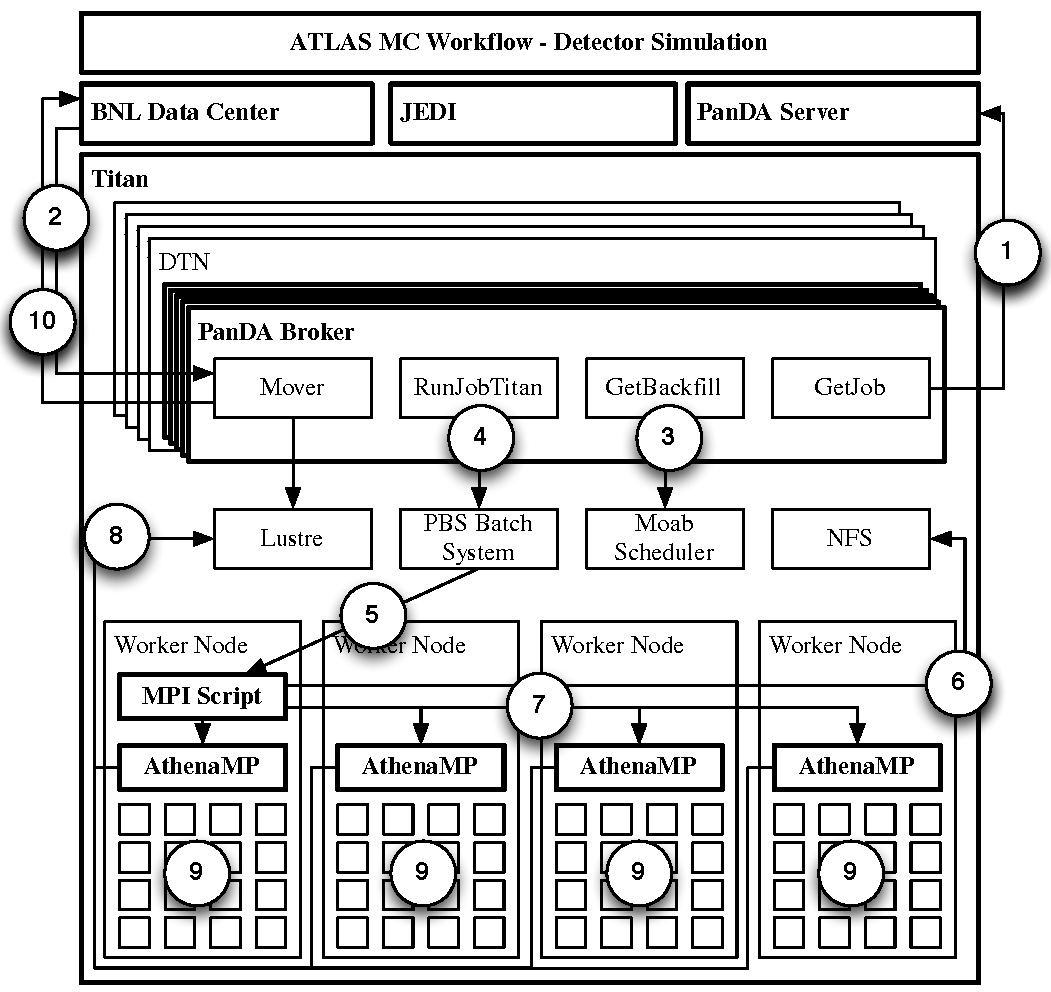
\includegraphics[width=\columnwidth]{figures/panda_broker_architecture.pdf}
    \caption{PanDA Broker architecture as deployed on Titan. Numbers indicates
    the execution process of a detector simulation job, part of the production
    ATLAS MD workflow. \jhanote{minor error in figure: "ATLAS MC" not "MD"}\mtnote{Fixed.}}
\label{fig:panda_broker}
\end{figure}

Backfill querying is performed via a dedicated Moab scheduler command while a
tailored Python MPI script is used to execute the payload of ATLAS jobs. This
MPI script enables the execution of unmodified Grid-centric, ATLAS jobs on
Titan. Typically, a MPI script is workload-specific as it sets up the execution
environment for a specific payload. This involves organization of worker
directories, data management, optional input parameters modification, and
cleanup on exit. Upon submission, a copy of the MPI script runs on every
available worker node,
% Each script knows its MPI rank (an index that runs from zero to a maximum
% number of nodes or script copies) as well as the total number of ranks in the
% current submission. When activated on worker nodes, each copy of the MPI
% script
starting the execution of the ATLAS job's payload in a subprocess and waits
until its completion.

MPI scripts are submitted to Titan's PBS batch system via
RADICAL-SAGA~\cite{radical-saga_url}, a Python module, compliant with the OGF
GFD.90 SAGA specification~\cite{goodale2008simple}. The Simple API for Grid
Applications (SAGA) offers a unified interface to diverse job schedulers and
file transferring services. In this way, SAGA provides an interoperability layer
that lowers the complexity of using distributed infrastructures. Behind the API
façade, RADICAL-SAGA implements a adaptor architecture: each adaptor interface
the SAGA API with different middleware systems and services, including the PBS
batch scheduler of Titan.

The data staging capabilities of the PanDA Broker are implemented via a file
system that is shared among DTNs and worker nodes. The input files with the
events of the ATLAS jobs are downloaded on the shared filesystem via the ATLAS
DDM service. The MPI script setup process includes making the location of these
files available to the payload of the ATLAS's jobs. The PanDA Broker can locate
the payload's output files on the shared filesystem and transfer them from Titan
to any computing center used by ATLAS.
% the ATLAS Tier 1 computing center at Brookhaven National Lab (BNL) or any
% other Grid site.

Once deployed on Titan, every PanDA Broker supports the execution of MC detector
simulation in 9 steps. PanDA Broker queries the Job Dispatcher module of the
PanDA server for ATLAS jobs that have been bound to Titan by JEDI
(Fig.~\ref{fig:panda_broker}:1). Upon receiving jobs descriptions, PanDA Broker
pulls jobs' input files from the ATLAS DDM service to the OLCF Lustre file
system (Fig.~\ref{fig:panda_broker}:3). PanDA Broker queries Titan's Moab
scheduler about current backfill availability (Fig.~\ref{fig:panda_broker}:2)
and creates an MPI script, wrapping enough ATLAS jobs' payload to fit backfill
availability. PanDA Broker submits the MPI script to the Titan's Torque batch
system via RADICAL-SAGA (Fig.~\ref{fig:panda_broker}:4).

Upon execution on the worker node(s) (Fig.~\ref{fig:panda_broker}:5), the MPI
script initializes and configures the execution environment
(Fig.~\ref{fig:panda_broker}:6), and executes one AthenaMP for each available
work node (Fig.~\ref{fig:panda_broker}:7). AthenaMP retrieves events from Lustre
(Fig.~\ref{fig:panda_broker}:8) and spawns 1 event simulation process on each of
the 16 available cores (Fig.~\ref{fig:panda_broker}:9).
% During execution, PanDA Broker monitors execution progress and sends PanDA
% Server ``heart beats'' for each job.; and (viii)
Upon completion of each MPI script, PanDA Broker transfer the jobs' output to
designated computing centre via the ATLAS DDM(Fig.~\ref{fig:panda_broker}:10),
and performs cleanup.

\mtnote{Address Alexei's comments: Add a paragraph explaining how this solution
has been ported to other HPC machines and reference relevant publications.}
While PanDA Broker implementation is resource specific, it was successfully
ported also to other supercomputers, including the Ansel (?) at \ldots and
\ldots at the National Energy Research Scientific Computing Center (NERSC).

% from the Job Dispatcher module of PanDA Server (as done by a PanDA Pilot);
% (iii) downloading events via PanDA Server's Data Service from ATLAS DDM to
% Titan's DTN; (iv) wrap the Geant4 payload into a PBS job; (v) submit jobs to
% Titan's PBS batch scheduler;

% Integration with Titan is the current focus for PanDA developers.

% The project aims to integrate Titan with the PanDA system using an updated
% PanDA Pilot that runs on the front-end node and submits ATLAS payloads to the
% worker nodes using the local batch system (PBS) via the SAGA (Simple API for
% Grid Applications) interface~\cite{SAGA}. This solves several complications
% of running on HPC worker nodes, including the lack of connectivity to outside
% world. The pilot can communicate with the PanDA server from the front-end
% machine.

% \paragraph*{HPC Backfill} HPC facilities are geared towards large scale jobs
% by design. Time allocation on an HPC is competitive and large projects are
% often preferred. About 10\% of capacity on a typical HPC machine is unused
% due to mismatches between job sizes and available resources. The worker nodes
% sit idle because there are not enough of them or they do not have enough time
% to handle a large scale computing job. On a machine of the scale of Titan,
% these 10\% correspond to estimated 300M core hours per year. A system that
% can occupy those temporarily free nodes with smaller scale tasks would be
% very valuable.

% This offers a great possibility for PanDA to harvest the opportunistic
% resources on Titan and use a similar mechanism on other HPCs. Functionality
% has been added to the PanDA Pilot to collect information about available
% unused worker nodes on Titan in real time.

% First test of the system were quite successful and show great promise in
% increasing the resource utilization on Titan.
